% Template:     Informe LaTeX
% Documento:    Archivo principal
% Versión:      8.3.8 (07/02/2025)
% Codificación: UTF-8
%
% Autor: Pablo Pizarro R.
%        pablo@ppizarror.com
%
% Manual template: [https://latex.ppizarror.com/informe]
% Licencia MIT:    [https://opensource.org/licenses/MIT]

% CREACIÓN DEL DOCUMENTO
\documentclass[
	spanish, % Idioma: spanish, english, etc.
	letterpaper, oneside
]{article}
\usepackage{amsmath}

% INFORMACIÓN DEL DOCUMENTO
\def\documenttitle {Métodos Neuronales para Regresión Simbólica}
\def\documentsubtitle {}
\def\documentsubject {Proyecto Inteligencia Computacional}

\def\documentauthor {Nombre del autor}
\def\coursename {Inteligencia Computacional}
\def\coursecode {EL-4106}

\def\universityname {Universidad de Chile}
\def\universityfaculty {Facultad de Ciencias Físicas y Matemáticas}
\def\universitydepartment {Departamento de Ingeniería Eléctrica}
\def\universitydepartmentimage {departamentos/die}
\def\universitydepartmentimagecfg {height=1.57cm}
\def\universitylocation {Santiago de Chile}

% INTEGRANTES, PROFESORES Y FECHAS
\def\authortable {
	\begin{tabular}{ll}
		Integrantes:
		& \begin{tabular}[t]{l}
			Benjamín Bruhn \\
			Mauricio González
		\end{tabular} \\
		Profesor:
		& \begin{tabular}[t]{l}
			Pablo Estevez
		\end{tabular} \\
		Auxiliar:
		& \begin{tabular}[t]{l}
			Pablo Cornejo
		\end{tabular} \\
		Ayudantes:
		& \begin{tabular}[t]{l}
			Diego Castillo\\
                Rodrigo Catalán\\ 
                Sebastián Guzmán\\ 
                Francisco Soto\\ 
                Bruno Araya\\ 
                Jorge Espejo
		\end{tabular} \\
		& \\
		\multicolumn{2}{l}{Fecha de entrega: \today} \\
		\multicolumn{2}{l}{\universitylocation}
	\end{tabular}
}

% IMPORTACIÓN DEL TEMPLATE
\input{config/template}

% INICIO DE PÁGINAS
\begin{document}

% PORTADA
\templatePortrait

% CONFIGURACIÓN DE PÁGINA Y ENCABEZADOS
%\templatePagecfg

% TABLA DE CONTENIDOS - ÍNDICE
\templateIndex

% CONFIGURACIONES FINALES
\templateFinalcfg

% ======================= INICIO DEL DOCUMENTO =======================

% ============================================================
\section{Introducción y Motivación}
% Contextualiza el problema: ¿por qué aprender ecuaciones?
% Qué limitaciones tienen las redes neuronales black-box.
% Relaciona con la búsqueda de modelos interpretables (EQL, Φ-SO, GINN-LP, etc.).
% Cita los papers [1]–[9] entregados con el enunciado del proyecto.

El descubrimiento automático de ecuaciones a partir de datos experimentales constituye un desafío central en la inteligencia computacional aplicada a las ciencias físicas y de la ingeniería. A diferencia de las aproximaciones empíricas o las redes neuronales convencionales de tipo \textit{black-box}, la regresión simbólica busca obtener expresiones analíticas explícitas que describan las relaciones subyacentes entre las variables del sistema, permitiendo interpretar los resultados, generalizar más allá del rango de entrenamiento y vincular las ecuaciones aprendidas con principios físicos conocidos.

Las redes neuronales tradicionales presentan una limitación fundamental en este contexto: si bien pueden alcanzar altos niveles de precisión, su estructura opaca impide comprender de manera directa qué relaciones han sido aprendidas, limitando su uso en entornos donde la interpretabilidad es esencial. En respuesta a este problema, se han desarrollado modelos orientados al aprendizaje simbólico de ecuaciones, donde la estructura de la red se define a partir de funciones matemáticas explícitas. Entre estos enfoques destaca el \textit{Equation Learner} (EQL) propuesto por Martius y Lampert~\cite{1}, el cual introduce capas con funciones elementales (\textit{id}, \textit{sin}, \textit{cos}, \textit{mult}) y un esquema de regularización basado en sparsity que induce representaciones algebraicamente compactas e interpretables. Este modelo ha sido posteriormente extendido a variantes como EQL$\div$~\cite{2}, que incorporan divisiones simbólicas para representar expresiones racionales.

En paralelo, otros enfoques como \textit{Physical Symbolic Optimization} (PhySO)~\cite{5} han propuesto integrar la búsqueda simbólica con principios físicos, restringiendo el espacio de soluciones mediante consistencia dimensional o información estructural conocida. Estos métodos combinan heurísticas simbólicas con aprendizaje automático para obtener expresiones más coherentes con las leyes de la física, sirviendo como un punto de comparación natural frente a modelos neuronales como EQL.

El presente proyecto se enmarca dentro de esta línea de investigación y tiene como propósito explorar la capacidad de los modelos neuronales de regresión simbólica para recuperar ecuaciones exactas y correlaciones físicas a partir de datos. Para ello, se utilizan los modelos EQL~\cite{1} y PhySO~\cite{5} sobre dos tipos de conjuntos de datos: (i) funciones sintéticas del benchmark de Nguyen~\cite{7}, con el objetivo de evaluar la precisión y la capacidad de extrapolación de las ecuaciones obtenidas, y (ii) datos experimentales asociados a los números de Nusselt, Reynolds y Prandtl provenientes de simulaciones CFD de baterías de litio~\cite{8,9}, con el fin de examinar la aplicabilidad de estos modelos en escenarios físicos reales. En conjunto, el estudio busca evaluar el potencial del EQL como herramienta base para el descubrimiento simbólico de ecuaciones, contrastando sus resultados con los de PhySO y analizando su capacidad para generar representaciones matemáticas interpretables y físicamente coherentes.




\newpage
% ============================================================
\section{Objetivos}
% Especifica el propósito global del trabajo.
% Ejemplo:
% Evaluar y comparar la capacidad del modelo EQL para descubrir ecuaciones exactas
% y correlaciones físicas a partir de datos experimentales.

\subsection*{Objetivo general del proyecto}
El objetivo general del proyecto es evaluar métodos neuronales de regresión simbólica para el descubrimiento de ecuaciones a partir de datos, con énfasis en el modelo \textit{Equation Learner} (EQL) y su capacidad de recuperar expresiones interpretables, cuantificar su desempeño (NRMSE y $R^2$) y analizar su comportamiento de extrapolación. El estudio considera validación sobre funciones sintéticas del benchmark de Nguyen y una aplicación preliminar sobre datos “reales” (p.\,ej., transferencia de calor en baterías o un modelo paramétrico de curvas de luz).

\subsection*{Objetivos específicos}
\begin{itemize}
    \item Implementar y adaptar los modelos EQL (en su versión original y división), DSR, Phy-so, Operon y Ginn-LP en un entorno de programación adecuado (p.\,ej., Python con TensorFlow/Keras).
    \item Generar y preparar conjuntos de datos sintéticos basados en las funciones de Nguyen para entrenamiento y validación.
    \item Entrenar los modelos sobre las funciones de Nguyen, optimizando una configuración de hiperparámetros (como número de capas, funciones activas y regularización) para cada modelo que fuera capas de funcionar con las 12 funciones.
    \item Evaluar el desempeño de los modelos extrapolando los datos fuera del rango de entrenamiento mediante métricas NRMSE y $R^2$ así como evaluando la similitud de la ecuación recuperada con la original, comparando los resultados de los modelos entre si.
    \item Aplicar los modelos a datos experimentales relacionados con transferencia de calor en baterías, evaluando su capacidad para descubrir correlaciones físicas relevantes.
    \item Documentar y presentar los resultados obtenidos, incluyendo las ecuaciones simbólicas descubiertas y su interpretación física.
\end{itemize}


\newpage
% ============================================================
\section{Descripción del Problema y Base de Datos}

\subsection{Datos sintéticos: Benchmark Nguyen}
% Describe las funciones usadas, sus rangos y propósito.
% Ejemplo:
% Se utilizan funciones Nguyen 1–10, definidas entre [-1,1] para entrenamiento y [-2,2] para prueba.
% Cada función presenta distintas combinaciones polinómicas y trigonométricas, permitiendo
% evaluar la capacidad simbólica del modelo.

Para llevar a cabo la implementación del proyecto serán necesarios, el desarrollo de bases de datos simples de los benckmarks de Nguyen \cite{3}, los que serán utilizados para medir el rendimiento de los distintos modelos frente a datos sintéticos. Habiendo terminado con estos, se podrá pasar a trabajar con los datos reales, para los que se escogieron los datos sobre baterías de litio relacionados al número de Nusselt\cite{9, 10}. \\

Los datos sintéticos son generados en el mismo código, apoyandose en la librería numpy para generar los datos base, usando la función linspace, luego guardando todos los datos complementandolo con las operaciones de python y numpy para generar las distintas ecuaciones de Nguyen. Estas fueron generadas en un intervalo de -1 a 1 para entrenamiento y -2 a 2 para validación para Nguyen 1 a 6, 9, 10, 11 y 12, 0 a 2 para entrenamiento y 0 a 4 para validación para Nguyen 7 y finalmente 0 a 4 para entrenamiento y 0 a 6 para validación para Nguyen 8, buscando extrapolar el trabajo hecho con el conjunto de entrenamiento.\\


\begin{figure}[h!]
  \centering % Comando para centrar dentro del entorno 'figure'
  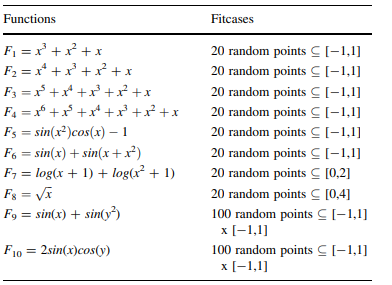
\includegraphics[width=0.6\textwidth]{Captura de pantalla 2025-10-20 191357.png}
  \caption{Tabla de funciones para regresión simbólica \cite{3}} % El título que va debajo
  \label{fig:mi_grafico} % La etiqueta para referenciarla
\end{figure}

Si bien en la imagen se especifícan 20 puntos aleatorios para las funciones 1 a 7 y 100 para las funciones 9 y 10. En este caso se utilizaron 1000 puntos para todas las simulaciones con un modelo y para el otro se usaron 100 puntos. Luego para la validación la cantidad de muestras se mantiene en 512 para el primer modelo

Los datos generados sintéticamente fueron entregados directamente al primer modelo (EQL) pero tuvieron que almacenarse en tensores de pytorch para el segundo modelo (Phy-SO).



\subsection{Datos reales: Baterías y transferencia térmica}
% Explica la fuente de los datos (De la Sotta, Hormazábal).
% Variables involucradas: Re, Pr, Nu, K o S.
% Describe el rango de valores, unidades y preprocesamiento (normalización, filtrado).

Luego los datos reales son tomados de un repositorio universitario, se trata de 4 archivos, de los mismos datos para distintas cantidades de celdas de baterías .tex que traen 4 columnas, cada una guardando un dato: K: separación de celdas, Rem: número de reynolds, prandtl: número de prandtl y nusselt: número de nusselt \cite{3}. 

Por el momento los datos de las baterías solo fueron entrenados con EQL. En esta parte del entrenamiento, erroneamente se concatenaron los datos de todas las configuraciones de celdas que se tenían (25, 53, 74 y 102), lo que alteró el entrenamiento. Además se ignoró la columna K ya que no se supo como formaba parte de la ecuación en el momento.\\


\newpage
% ============================================================
\section{Metodología y Arquitecturas}

\subsection{Equation Learner (EQL) y Equation Learner with Division (EQL-Div)}
% Explica la estructura del modelo:
% - Capas simbólicas (funciones: id, sin, cos, mult, sig).
% - Pesos W y sesgos b como coeficientes de la ecuación.
% - Fases de entrenamiento: T₀ (warm-up), T₁ (sparsity L1), T₂ (fine-tune L0).
% - Parámetros controlados: número de capas, funciones excluidas, lambda (regularización).

El método \textit{Equation Learner} (EQL) propuesto por Martius y Lampert~\cite{1}, junto con su extensión para funciones racionales (\textbf{EQL-Div}) presentada por Sahoo et al.~\cite{2}, corresponde a una arquitectura neuronal diseñada específicamente para la regresión simbólica, cuyo objetivo es aprender ecuaciones interpretables a partir de datos. A diferencia de las redes neuronales tradicionales, estos modelos no buscan aproximar valores mediante combinaciones no lineales arbitrarias, sino que restringen sus operaciones a un conjunto de funciones matemáticas elementales (identidad, seno, coseno, multiplicación y, en el caso de EQL-Div, división). Esto permite que la red reconstruya expresiones analíticas exactas, incluyendo leyes físicas racionales, y generalice eficazmente más allá del dominio de entrenamiento.

La implementación se realizó en \texttt{Python} empleando la librería \texttt{TensorFlow}, basándose en la estructura del repositorio oficial (\texttt{EQL-TensorFlow})~\cite{3} con modificaciones de compatibilidad para Python~3.12 y ejecución en GPU en Google~Colab.

\subsubsection{Arquitectura del modelo}

Tanto EQL como EQL-Div están compuestos por una secuencia de \textbf{capas simbólicas}, donde cada capa aplica un conjunto de funciones sobre las salidas de la anterior. 
Cada capa $l$ genera una salida $y^{(l)}$ a partir de las entradas $x^{(l-1)}$ según:
\begin{equation}
    y^{(l)} = f\!\left(W^{(l)} x^{(l-1)} + b^{(l)}\right),
\end{equation}
donde $W^{(l)}$ y $b^{(l)}$ corresponden a los pesos y sesgos de la capa $l$, y $f(\cdot)$ representa el conjunto de activaciones simbólicas. 
Para el EQL estándar, este conjunto se define como:
\[
\mathcal{F}_{EQL} = \{\, id(x),\; \sin(x),\; \cos(x),\; \sigma(x),\; x_i \cdot x_j \,\}.
\]
En el caso de \textbf{EQL-Div}, el conjunto se expande para incluir la operación binaria de división~\cite{2}:
\[
\mathcal{F}_{Div} = \mathcal{F}_{EQL} \cup \left\{ \frac{x_i}{x_j} \right\}.
\]
Estas funciones permiten que la red construya expresiones complejas, tales como términos trigonométricos anidados o, en el caso de EQL-Div, relaciones inversas del tipo:
\[
\sin(x_1^2),\quad \frac{x_1 \cdot x_2}{x_3 + c},\quad \cos(x_1) + x_2^{-1}.
\]

El número de combinaciones posibles por capa está determinado por la configuración de la red (ancho de capa), que controla cuántas unidades binarias y unarias se construyen. 
Así, la arquitectura regula la capacidad simbólica del modelo: valores altos permiten combinaciones más complejas, mientras que valores bajos inducen ecuaciones más simples.

\begin{figure}[H]
    \centering
    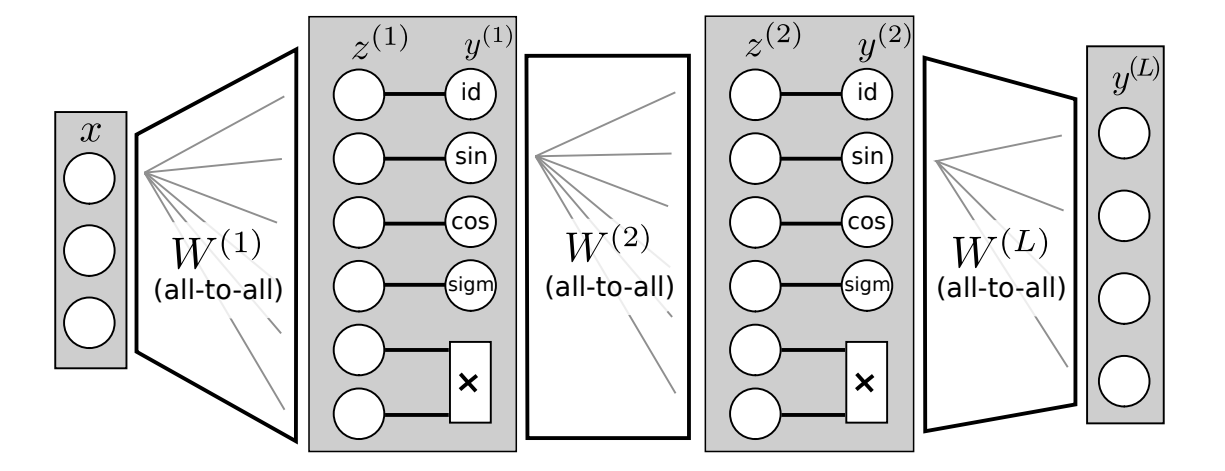
\includegraphics[width=0.85\textwidth]{img/EQL.png}
    \caption{Arquitectura general del modelo \textit{Equation Learner} (EQL). El esquema ilustra el flujo de información a través de capas simbólicas. En la variante EQL-Div, las unidades de multiplicación se complementan con unidades de división, permitiendo la formación de denominadores.}
    \label{fig:eql_architecture}
\end{figure}

\subsubsection{Fases de entrenamiento y regularización}

El entrenamiento de estos modelos se realiza en tres fases consecutivas que controlan la complejidad y parsimonia de la ecuación resultante. Para EQL-Div, se añade un mecanismo crítico de estabilidad numérica:

\begin{enumerate}
    \item \textbf{Fase $T_0$ (Warm-up):} entrenamiento inicial sin regularización, donde los pesos se ajustan libremente para explorar el espacio de funciones.
    \item \textbf{Fase $T_1$ (Sparsity – L$_1$):} se aplica penalización L$_1$ sobre los pesos para inducir \textit{sparsity}, forzando que muchos de ellos se vuelvan cero. 
    Esta etapa elimina conexiones y funciones irrelevantes, reduciendo la ecuación a su forma esencial.
    \item \textbf{Fase $T_2$ (Fine-tune – L$_0$):} se mantienen fijos los pesos de magnitud pequeña ($|w|<\varepsilon$) y se continúa el entrenamiento con regularización suave tipo L$_0$. 
    Esto refina los coeficientes finales de los términos relevantes y entrega una ecuación simbólicamente estable.
\end{enumerate}

Adicionalmente, el modelo **EQL-Div** implementa una penalización específica para evitar singularidades (divisiones por cero), descartando o castigando fuertemente las soluciones donde el denominador tiende a cero dentro del dominio de los datos~\cite{2}.
Durante la fase final se aplica un umbral de redondeo \texttt{atol} (o \texttt{threshold}) que fuerza explícitamente a cero los pesos pequeños, consolidando la estructura final del modelo.


\subsubsection{Aspectos de implementación y programación}

El desarrollo del proyecto se llevó a cabo utilizando y adaptando el repositorio oficial de \textit{Equation Learner} (EQL) propuesto por Kristof~Pusztai\footnote{\url{https://github.com/KristofPusztai/EQL}}, implementado en \texttt{TensorFlow/Keras}. 
Sobre esta base, se incorporaron rutinas auxiliares y scripts propios que permitieron realizar los experimentos tanto con funciones sintéticas del benchmark de Nguyen como con los datos experimentales del número de Nusselt.\\ 

\textbf{Configuración de Hiperparámetros:}
El entrenamiento se configuró para EQL normal con los siguientes parámetros base, identificados en el script de ejecución:
\begin{itemize}
    \item \textbf{Épocas (\texttt{num\_epochs}):} 10000, repartidas en la estructura 0-25\%-95\%-100\% que se recomienda en la literatura.
    \item \textbf{Capas (\texttt{capas}):} Se utilizó una estructura de 3 capas ocultas con una distribución de ancho 1-2-1. Buscano poder encontrar todas las configuraciones de Nguyen.
    \item \textbf{Lambda y atol} (\texttt{lambda}, \texttt{atol}): Se utilizaron valores de 0.001 y 0.0001 respectivamente, los cuales se mantuvieron constantes en todos los experimentos.
\end{itemize}

Para EQL-Div, se emplearon parámetros similares, ajustando el número de épocas a 8000, las capas utilizadas fueron 3 pero para algunas funciones se uso amplitud 1 y otras 2 (en EQL division se puede configurar una unica amplitud para todas las capas), esto due adaptado según la complejidad de las funciones trabajadas, además se mantuvieron los mismos valores de lambda y atol.\\






\subsection{Physical Symbolic Optimization (Φ-SO)}
% Explica la estructura del modelo:

El método Physical Symbolic Optimization (Φ-SO), propuesto por Tenachi et al.~\cite{2}, es un entorno diseñado para la regresión simbólica, enfocado en recuperar expresiones analíticas a partir de datos físicos. A diferencia de otros métodos que exploran un vasto espacio de funciones, Φ-SO integra el análisis dimensional como un componente central de su proceso de búsqueda. El sistema está construido para proponer únicamente soluciones donde las unidades físicas son consistentes por construcción, eliminando expresiones físicamente imposibles y restringiendo enormemente el espacio de búsqueda.

El modelo se implementó en \texttt{Python} utilizando la librería \texttt{PyTorch}. Su enfoque se basa en técnicas de aprendizaje por refuerzo profundo (Deep Reinforcement Learning) para aprender y aplicar las restricciones de unidades durante la generación de ecuaciones.

\subsubsection{Arquitectura y generación de expresiones}

El núcleo de Φ-SO es una Red Neuronal Recurrente (RNN) que genera expresiones simbólicas. Las ecuaciones se representan como secuencias de símbolos (tokens) en notación prefija (Polish notation). En cada paso de la generación, la RNN recibe información contextual sobre la expresión parcial que se está construyendo, incluyendo el token padre, el token hermano y, fundamentalmente, las unidades físicas requeridas para el siguiente token.

La RNN produce una distribución de probabilidad categórica sobre toda la biblioteca de tokens disponibles (operadores, variables, constantes). La innovación clave es la aplicación de un "prior de unidades físicas" sobre esta distribución. Este prior actúa como una máscara que anula la probabilidad de seleccionar tokens que violarían la coherencia dimensional de la ecuación. De este modo, la red aprende activamente las reglas del análisis dimensional y solo explora soluciones físicamente viables.

\begin{figure}[H]
    \centering
    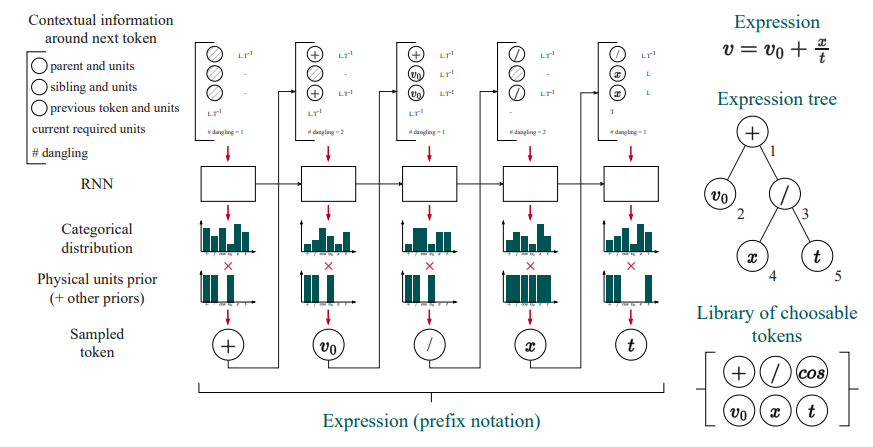
\includegraphics[width=0.9\textwidth]{PhySO.png}
    \caption{Esquema de generación de expresiones en Φ-SO. La RNN recibe información contextual (incluyendo unidades) y genera una distribución de probabilidad. Un prior de unidades físicas filtra esta distribución antes de muestrear el siguiente token. Adaptado de \cite{2}.}
    \label{fig:physo_architecture}
\end{figure}

\subsubsection{Entrenamiento por Aprendizaje por Refuerzo}

A diferencia del entrenamiento por fases de EQL, Φ-SO utiliza una estrategia de aprendizaje por refuerzo. El proceso no se divide en etapas de regularización, sino que se optimiza mediante un gradiente de política (policy gradient) de tipo "risk-seeking" (búsqueda de riesgo). El entrenamiento sigue un ciclo iterativo:

\begin{enumerate}
    \item \textbf{Generación:} La RNN (el agente) muestrea un lote de expresiones (acciones) candidatas, guiada por el prior de unidades.
    \item \textbf{Evaluación:} Para cada expresión generada, se optimizan sus constantes libres para ajustar los datos de entrada.
    \item \textbf{Recompensa:} Se calcula una recompensa (reward) para cada expresión, basada en su precisión de ajuste (por ejemplo, $R^2$).
    \item \textbf{Actualización:} El gradiente de política utiliza estas recompensas para actualizar los pesos de la RNN, incrementando la probabilidad de generar expresiones de alta recompensa (alta precisión y dimensionalmente correctas) en futuras iteraciones.
\end{enumerate}

El resultado final del proceso es un conjunto de expresiones en la frontera de Pareto, que balancean la complejidad de la ecuación y la precisión del ajuste a los datos.


\subsubsection{Aspectos de implementación y programación}

Para la implementación se utilizó el paquete oficial \texttt{physo} (Physical Symbolic Optimization)\footnote{\url{https://github.com/WassimTenachi/PhySO}}, el cual está basado en la librería \texttt{PyTorch}. El trabajo se condujo en un notebook de Google Colab, donde se cargaron los datos experimentales del número de Nusselt y se ejecutó el proceso de aprendizaje por refuerzo para encontrar la ecuación gobernante. Los principales procesos realizados fueron:

\begin{itemize}
    \item \textbf{Carga y preparación de datos:}
    Se empleó la librería \texttt{pandas} para importar el archivo \texttt{NN\_data.csv}. De este, se extrajeron las variables de interés (Reynolds \texttt{Re}, Prandtl \texttt{Pr} y Nusselt \texttt{Nu\_D}). Se especificaron sus unidades físicas (adimensionales) y se procedió a separar los datos en conjuntos de entrenamiento y prueba.

    \item \textbf{Definición de la biblioteca y configuración:}
    Se definió la biblioteca de funciones (\texttt{my\_tokens}) que el agente podía utilizar. Esta incluyó operadores aritméticos (\texttt{add}, \texttt{mul}, \texttt{div}, \texttt{inv}, \texttt{n2}, \texttt{sqrt}), funciones (\texttt{exp}, \texttt{log}) y constantes libres (\texttt{c}). El entorno se configuró a través de un diccionario \texttt{config}, donde se ajustaron los parámetros del prior de unidades (análisis dimensional), la función de recompensa (\texttt{reward.SquashedNRMSE}) y los hiperparámetros del algoritmo de aprendizaje (\texttt{gamma}, \texttt{entropy\_weight}).

    \item \textbf{Entrenamiento por Aprendizaje por Refuerzo:}
    El proceso de búsqueda se inició con la función \texttt{physo.fit}, proporcionando los datos, unidades y la configuración. A diferencia de EQL, el entrenamiento no ocurre en fases, sino que \texttt{physo} aplica su algoritmo de gradiente de política para explorar el espacio de ecuaciones. Este proceso optimiza la recompensa (basada en NRMSE) hasta alcanzar un tiempo máximo de ejecución (\texttt{max\_time\_seconds}).

    \item \textbf{Evaluación y visualización de resultados:}
    Al finalizar la ejecución, se extrajeron las mejores expresiones desde la "Sala de la Fama" (\texttt{hall\_of\_fame\_PhysicalExpression}). Se tomó la mejor expresión candidata para obtener su fórmula simbólica (\texttt{best\_expression.formula}) y se evaluó su desempeño con las métricas RMSE y $R^2$ sobre los datos de prueba. Se utilizaron las herramientas del paquete (\texttt{physo.viz}) para graficar la frontera de Pareto (\texttt{plot\_HOF}) y la comparativa entre valores reales y predichos (\texttt{plot\_expression}).
\end{itemize}

Todo el proceso se desarrolló en Google Colab, garantizando la reproducibilidad del experimento mediante la instalación de la librería \texttt{physo} y el uso del mismo conjunto de datos experimentales.


\subsection{Growing Interpretable Neural Network (GINN-LP)}

El método GINN-LP (Growing Interpretable Neural Network for Laurent Polynomials), propuesto recientemente por Ranasinghe et al. \cite{}, representa un enfoque híbrido que combina la flexibilidad de las redes neuronales con una estructura fuertemente restringida para la búsqueda de polinomios de Laurent multivariables. A diferencia de EQL, que explora un espacio de funciones generales (seno, coseno, etc.), GINN-LP se especializa en descubrir expresiones de la forma:

\begin{equation}
    f(\mathbf{x}) = \sum_{k=1}^{K} c_k \prod_{i=1}^{D} x_i^{p_{ki}}
\end{equation}

donde $c_k$ son coeficientes reales y $p_{ki}$ son potencias enteras (positivas o negativas). Esta especialización lo hace particularmente robusto para problemas físicos donde las leyes de potencias y las relaciones polinomiales son predominantes, como es el caso de las correlaciones de números adimensionales (Nusselt, Reynolds).

\subsubsection{Arquitectura y Algoritmo de Crecimiento}

La arquitectura de GINN-LP no es estática; utiliza un algoritmo de crecimiento (growing algorithm) que ajusta la complejidad del modelo a los datos. El proceso consta de dos mecanismos principales:

\begin{enumerate}
    \item \textbf{Optimización de Parámetros:} Para una estructura fija (número de términos $K$), la red optimiza tanto los coeficientes $c_k$ como los exponentes $p_{ki}$ mediante descenso de gradiente. Una característica distintiva es que los exponentes se relajan a valores continuos durante el entrenamiento y se discretizan posteriormente para recuperar la forma simbólica exacta.
    
    \item \textbf{Crecimiento Estructural:} El modelo comienza con una estructura simple y añade nuevos términos ("bloques" neuronales que representan monomios) iterativamente si el error de ajuste no satisface un criterio de convergencia. Esto permite que el modelo encuentre el equilibrio entre parsimonia (pocos términos) y precisión, evitando el sobreajuste típico de polinomios de alto grado.
\end{enumerate}

\subsubsection{Aspectos de implementación y configuración}

Para este proyecto, se utilizó la librería oficial \texttt{ginnlp} en Python. La implementación se integró al flujo de trabajo existente, adaptando los scripts de entrenamiento para manejar tanto las funciones sintéticas de Nguyen como los datos experimentales de baterías.

\textbf{Pre-procesamiento de datos:}
Un aspecto crítico observado durante la implementación fue la sensibilidad del modelo al dominio de entrada, especialmente para exponentes fraccionarios o negativos. Basado en los scripts de experimentación (\texttt{run\_nguyen\_train.py}), se aplicó un desplazamiento (shift) a las variables de entrada:
\begin{equation}
    X_{input} = X_{raw} + \delta
\end{equation}
donde $\delta = 1.1$ para los benchmarks de Nguyen. Este desplazamiento asegura que las entradas sean estrictamente positivas, evitando singularidades en el origen o errores de dominio en potencias fraccionarias, facilitando la convergencia del gradiente.

\textbf{Configuración de Hiperparámetros:}
El entrenamiento se configuró con los siguientes parámetros base, identificados en el script de ejecución:
\begin{itemize}
    \item \textbf{Épocas (\texttt{num\_epochs}):} 250, permitiendo suficiente tiempo para la estabilización de los pesos.
    \item \textbf{Iteraciones de entrenamiento (\texttt{train\_iter}):} 3, controlando los ciclos de refinamiento de la estructura.
    \item \textbf{Optimización:} Se utilizó el optimizador interno de la librería, el cual gestiona la cuantización de los exponentes para recuperar la ecuación simbólica final (\texttt{model.recovered\_eq}).
\end{itemize}

Para la evaluación, las ecuaciones recuperadas fueron evaluadas utilizando un entorno numérico estándar (\texttt{numpy}), asegurando que las métricas de NRMSE y $R^2$ fueran comparables con las obtenidas mediante EQL y PhySO.

\subsection{Operon (C++ Symbolic Regression Framework)}

En este trabajo se utilizó \textbf{Operon}, un framework de Regresión Simbólica de alto rendimiento desarrollado en C++ moderno, diseñado específicamente para manejar grandes poblaciones y ejecuciones prolongadas con una eficiencia computacional superior a las implementaciones tradicionales basadas en Python puro.

\subsubsection{Arquitectura y Codificación Lineal}

A diferencia de los enfoques clásicos de Programación Genética (GP) que representan las expresiones matemáticas como árboles de objetos enlazados mediante punteros, Operon implementa una \textbf{codificación lineal} (linear encoding). 

En esta arquitectura, los árboles sintácticos se representan como arreglos contiguos en memoria utilizando notación postfija (Reverse Polish Notation). Esta decisión de diseño tiene dos ventajas críticas para el rendimiento:
\begin{itemize}
    \item \textbf{Localidad espacial:} Al ser memoria contigua, se maximiza el uso de la caché del procesador, reduciendo drásticamente los fallos de caché (cache misses) durante la evaluación.
    \item \textbf{Evaluación vectorizada:} Permite el uso eficiente de instrucciones SIMD y paralelismo a nivel de datos para evaluar miles de individuos simultáneamente.
\end{itemize}

\subsubsection{Algoritmo Evolutivo y Selección de Pareto}

El núcleo del algoritmo es un proceso evolutivo generacional. Sin embargo, para mitigar el problema del \textit{bloat} (crecimiento descontrolado de la complejidad de las fórmulas sin ganancia significativa de precisión), nuestra metodología se alejó de la minimización del error cuadrático medio (MSE) como único objetivo.

En su lugar, se implementó una estrategia de selección multiobjetivo basada en el \textbf{Frente de Pareto} , optimizando simultáneamente dos variables en conflicto:
\begin{enumerate}
    \item \textbf{Precisión:} Minimizando el RMSE (Root Mean Squared Error).
    \item \textbf{Simplicidad:} Minimizando la longitud del árbol (número de nodos).
\end{enumerate}

Esta estrategia, fundamentada en el principio de parsimonia (Navaja de Ockham), permitió seleccionar modelos que ofrecen el mejor equilibrio teórico, descartando aproximaciones complejas (como series de Taylor truncadas) en favor de las estructuras analíticas exactas subyacentes.

\subsubsection{Aspectos de implementación y configuración}

La implementación se realizó utilizando la interfaz de Python \texttt{pyoperon}, integrando el núcleo de C++ con el flujo de trabajo de análisis de datos en Python. Un desafío técnico crítico abordado fue la interoperabilidad de memoria: se implementó una sanitización estricta de los datos de entrada, forzando arreglos \texttt{C-contiguous} de doble precisión (\texttt{float64}) para evitar errores de segmentación y garantizar la correcta lectura de variables ($X_1, X_2, \dots$) por parte del motor de C++.

La configuración experimental utilizada para los benchmarks de Nguyen y los casos reales se detalla en la Tabla \ref{tab:params_operon}.

\begin{table}[H]
\centering
\caption{Configuración de hiperparámetros para Operon.}
\label{tab:params_operon}
\begin{tabular}{|l|l|}
\hline
\textbf{Parámetro} & \textbf{Valor / Configuración} \\ \hline
Tamaño de Población & 3000 individuos \\ \hline
Generaciones & 4000 \\ \hline
Límite de Longitud ($L_{max}$) & 25 nodos  \\ \hline
Optimización Numérica & 10 iteraciones \\ \hline
\end{tabular}
\end{table}


\subsection{Configuración experimental}
% Describe cómo se entrenaron los modelos:
% - Número de muestras por función (Nguyen).
% - Valores de lambda, learning rate, batch size.
% - Semilla aleatoria (para reproducibilidad).
% - Herramientas usadas (Python, TensorFlow/Keras, Google Colab, GPU local).

Se realizaron los experimentos sobre el conjunto de funciones sintéticas del benchmark de Nguyen~(1--12). Cada función fue entrenada en el rango $[-1,1]$ y evaluada en el rango extendido $[-2,2]$. 



\subsection{Métricas de evaluación}

La evaluación del modelo se realiza mediante la comparación entre los valores predichos y los valores reales de cada dataset, tanto para los conjuntos sintéticos de Nguyen como para los datos experimentales del número de Nusselt. Los modelos se entrenan con datos normalizados (media cero y varianza unitaria) y se validan utilizando un 80\% de las muestras para entrenamiento y un 20\% para prueba, lo que permite analizar el comportamiento del modelo en condiciones de extrapolación.

Las métricas utilizadas para cuantificar el desempeño fueron el error cuadrático medio normalizado (NRMSE) y el coeficiente de determinación ($R^2$), definidos como:
\begin{equation}
NRMSE = \frac{\sqrt{\text{MSE}(y,\hat{y})}}{y_{\max}-y_{\min}}, 
\qquad
R^2 = 1 - \frac{\sum(y-\hat{y})^2}{\sum(y-\bar{y})^2}.
\end{equation}

Estas métricas permiten evaluar tanto la fidelidad del ajuste como la capacidad de generalización del modelo. 
Además, se generaron visualizaciones gráficas que muestran la comparación entre los valores reales y los valores predichos, representadas en forma de dispersión y en curvas de ajuste. Estas gráficas permiten observar el grado de alineación con la diagonal ideal ($y = \hat{y}$) y facilitan la interpretación cualitativa del desempeño del modelo.

Asimismo, el modelo entrega de manera automática la \textbf{fórmula simbólica obtenida} mediante el método interno \texttt{model.formula()}, el cual reconstruye la ecuación aprendida a partir de los pesos no nulos en cada capa. De esta forma, junto con las métricas de error y las gráficas de ajuste, se reporta la ecuación final descubierta por el EQL, lo que permite interpretar directamente la relación funcional aprendida por la red. 

Para los casos experimentales de Nusselt, se añadieron representaciones en función del número de Reynolds y del parámetro geométrico $S$, ---

\newpage
% ============================================================
\section{Resultados}

\subsection{Funciones Nguyen}
% Incluye tablas con métricas NRMSE y R² para Nguyen-1 a Nguyen-10.
% Muestra ejemplos de ecuaciones recuperadas y sus gráficos.

Los modelos considerados fueron evaluados utilizando el conjunto de funciones del benchmark de Nguyen, con el objetivo de analizar su capacidad para recuperar ecuaciones en distintos niveles de complejidad. Para cada modelo se obtuvieron las métricas de desempeño correspondientes, las cuales se presentan de manera individual en las tablas incluidas en el Anexo, junto con los gráficos asociados a cada función del benchmark. Estas visualizaciones permiten apreciar el ajuste obtenido por cada método y la consistencia de las expresiones recuperadas respecto de los datos sintéticos. En conjunto, los resultados permiten comparar el comportamiento global de las distintas aproximaciones de regresión simbólica, destacando sus diferencias en precisión, estabilidad y capacidad de generalización.

Los modelos considerados fueron evaluados utilizando el conjunto de funciones del benchmark de Nguyen, con el objetivo de analizar su capacidad para recuperar ecuaciones en distintos niveles de complejidad. Para cada modelo se obtuvieron las métricas de desempeño correspondientes, las cuales se presentan de manera individual en las tablas incluidas en el Anexo, junto con los gráficos asociados a cada función del benchmark. De forma adicional, se aplicó la misma metodología al caso de baterías, evaluando el ajuste de los modelos sobre los datos termodinámicos y fluidodinámicos asociados, cuyos resultados también se encuentran detallados en el Anexo. En conjunto, estas evaluaciones permiten comparar el comportamiento global de las distintas aproximaciones de regresión simbólica, destacando sus diferencias en precisión, estabilidad y capacidad de generalización en ambos escenarios de estudio.



TIRARÍA TODO ESTO PARA EL ANEXO.

 La Tabla~\ref{tab:nguyen_metrics_6models} presenta los valores de error cuadrático medio normalizado (NRMSE) y coeficiente de determinación ($R^2$) obtenidos en el conjunto de prueba para ambos modelos.

\begin{table}[H]
    \centering
    \caption{Métricas de desempeño de los 6 modelos (EQL, EQL-Div, Phy-SO, Ginn-LP, DSR, Operon) sobre funciones de Nguyen seleccionadas.}
    \label{tab:nguyen_metrics_6models}
    \resizebox{\textwidth}{!}{% Ajusta la tabla al ancho del texto
    \begin{tabular}{lcccccccccccc}
        \toprule
        \multirow{2}{*}{\textbf{Función}} & \multicolumn{2}{c}{\textbf{EQL}} & \multicolumn{2}{c}{\textbf{EQL-Div}} & \multicolumn{2}{c}{\textbf{Phy-SO}} & \multicolumn{2}{c}{\textbf{Ginn-LP}} & \multicolumn{2}{c}{\textbf{DSR}} & \multicolumn{2}{c}{\textbf{Operon}} \\ 
        \cmidrule(lr){2-3} \cmidrule(lr){4-5} \cmidrule(lr){6-7} \cmidrule(lr){8-9} \cmidrule(lr){10-11} \cmidrule(lr){12-13}
        & \textbf{NRMSE} & \textbf{$R^2$} & \textbf{NRMSE} & \textbf{$R^2$} & \textbf{NRMSE} & \textbf{$R^2$} & \textbf{NRMSE} & \textbf{$R^2$} & \textbf{NRMSE} & \textbf{$R^2$} & \textbf{NRMSE} & \textbf{$R^2$} \\ 
        \midrule
        Nguyen-3 & 0.078 & 0.906 & 0.065 & 0.875 & 0.007 & 0.999 & 0.099 & 0.990 & 0 & 1.000 & 0 & 1.000 \\
        Nguyen-5 & 0.738 & -3.459 & 0.495 & -1.201 & 0.009 & 0.997 & 0.978 & 0.041 & 0.000 & 0.999 & 0.000 & 0.999 \\
        Nguyen-7 & 0.669 & -4.895 & 0.053 & 0.968 & 0.005 & 0.999 & 0.173 & 0.969 & 0.000 & 0.999 & 0.000 & 0.999 \\
        Nguyen-8 & 0.107 & 0.852 & 0.925 & 0.073 & 0.000 & 0.999 & 0.026 & 0.999 & 0.000 & 0.999 & 0.000 & 0.999 \\
        Nguyen-10 & 0.052 & 0.955 & 0.014 & 0.997 & 0.025 & 0.986 & 0.160 & 0.974 & 0.000 & 0.999 & 0.000 & 0.999 \\
        Nguyen-12 & 0.169 & 0975 & 0.132 & 0.485 & 0.057 & 0.953 & 0.189 & 0.963 & 0.073 & 0.913 & 0.000 & 0.999 \\
        \bottomrule
    \end{tabular}
    }
\end{table}



\subsection{Caso de Baterías}
% Explica los resultados sobre los datos experimentales.
% Muestra el gráfico Nu vs Re (similar a Figura 3.2 del in


Se abordó el problema de regresión para los datos experimentales de baterías, buscando una correlación para el número de Nusselt ($\text{Nu}$) en función de Reynolds ($\text{Re}$) y Prandtl ($\text{Pr}$). El análisis se divide en los resultados de referencia de la literatura y los obtenidos mediante la implementación propia del modelo EQL.

\subsubsection{Resultados de Referencia (Tesis [2])}

Como punto de referencia para el ajuste de datos, se utilizaron los resultados presentados en la tesis de De la Sotta [2]. Este trabajo establece un \textit{benchmark} de desempeño para este conjunto de datos específico.

Las métricas de error reportadas en [2] para el mejor modelo encontrado son:
\begin{itemize}
    \item \textbf{MSE In-Sample (Entrenamiento):} 2.946886
    \item \textbf{MSE Out-of-Sample (Prueba):} 15.902144
\end{itemize}

Visualmente, el ajuste (Figura~\ref{fig:ref_nusselt_results}) muestra un coeficiente de determinación $R^2$ de $0.979$ para los datos de entrenamiento (IN) y $R^2$ de $0.887$ para los de prueba (OUT).

\begin{figure}[H]
    \centering
    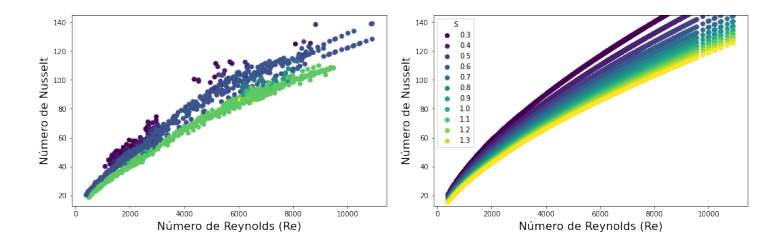
\includegraphics[width=1.0\textwidth]{Captura de pantalla 2025-10-20 184649.png}
    \caption{Resultados de referencia reportados en De la Sotta [2]. Izquierda: Correlación log-log. Derecha: Gráfico de paridad.}
    \label{fig:ref_nusselt_results}
\end{figure}

\subsubsection{Resultados Obtenidos (Implementación EQL)}

De forma paralela, se aplicó el modelo \textbf{\textit{Equation Learner} (EQL)} a los mismos datos. Este enfoque utiliza una red neuronal simbólica para \textit{descubrir} la estructura de la ecuación desde cero, en lugar de solo optimizar coeficientes.

Los resultados de la mejor expresión simbólica encontrada por la implementación de EQL se muestran en la Figura~\ref{fig:eql_nusselt_results}.

\begin{itemize}
    \item El gráfico de paridad (derecha) muestra un ajuste preciso para los datos de entrenamiento (círculos azules) y una dispersión controlada para los datos de prueba (cruces naranjas), sugiriendo una buena capacidad de generalización.
    \item La correlación $\text{Nu}$ vs. $\text{Re}$ (izquierda) también demuestra que la ecuación descubierta por EQL captura exitosamente la tendencia física de los datos de CFD (círculos negros).
\end{itemize}

El desempeño visual del EQL es robusto y comparable al \textit{benchmark} de referencia, validando este enfoque como una alternativa capaz de descubrir la forma funcional de la correlación directamente desde los datos.

\begin{figure}[H]
    \centering
    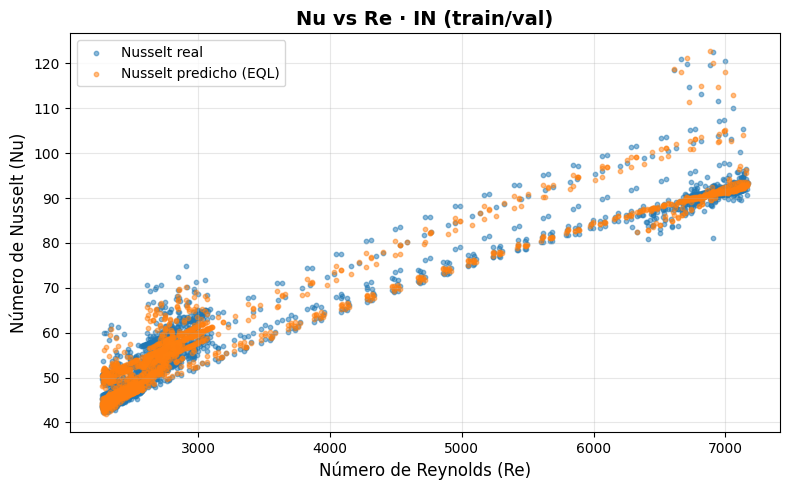
\includegraphics[width=1.0\textwidth]{NUvsREYNOLDS25.png}
    \caption{Resultados obtenidos con la implementación propia de EQL sobre los datos de baterías. Izquierda: Correlación log-log $\text{Nu}$ vs. $\text{Re}$. Derecha: Gráfico de paridad (Train/Test).}
    \label{fig:eql_nusselt_results}
\end{figure}



\newpage
% ============================================================
\section{Discusión}
% Analiza los resultados:
% - Qué tan bien recupera EQL las ecuaciones teóricas.
% - Cómo influyen los hiperparámetros (capas, funciones excluidas, lambda).
% - Ventajas del enfoque simbólico frente a redes tradicionales.
% - Limitaciones observadas: lentitud, sensibilidad, ruido.



\newpage
% ============================================================
\section{Plan de Trabajo Restante}
% Lista de tareas pendientes y cronograma estimado.
% Ejemplo:
\begin{itemize}[label=--]
    \item Extender EQL a variantes con divisiones (EQL÷).
    \item Ajustar correlación Nusselt con inclusión de \(Pr\).
    \item Comparar con otro método simbólico (DSR o GINN-LP).
    \item Preparar informe final y análisis comparativo.
\end{itemize}




\newpage
% ============================================================
\section{Conclusiones Preliminares}
% Resume los hallazgos más importantes.
% - El modelo EQL logra alta precisión y recupera ecuaciones exactas.
% - Presenta extrapolación robusta.
% - Es aplicable a datos físicos con coherencia dimensional.


\newpage
\bibliography{library}
\newcommand{\figuraNguyen}[1]{
    \begin{figure}[H] % H fuerza la posición aquí
        \centering
        
        % --- FILA 1: EQL, EQL-DIV, DSR (Rutas conocidas) ---
        \begin{subfigure}[b]{0.5\textwidth}
            \centering
            % Ajusta la extensión (.png, .jpg, .pdf) si es necesario
            \includegraphics[width=\linewidth]{"Fotos Proyecto/EQL/Nguyen-#1"} 
            \caption{EQL}
        \end{subfigure}
        \hfill
        \begin{subfigure}[b]{0.5\textwidth}
            \centering
            \includegraphics[width=\linewidth]{"Fotos Proyecto/EQL-DIV/Nguyen-#1"}
            \caption{EQL-Div}
        \end{subfigure}
        \hfill
        \begin{subfigure}[b]{0.5\textwidth}
            \centering
            \includegraphics[width=\linewidth]{"Fotos Proyecto/DSR/Nguyen-#1"}
            \caption{DSR}
        \end{subfigure}
        
        \vspace{1em} % Espacio vertical entre filas
        
        % --- FILA 2: Phy-so, Ginn-Lp, Operon (Rutas asumidas) ---
        % NOTA: Debes verificar que estas carpetas existan o cambiar la ruta aquí
        %\begin{subfigure}[b]{0.5\textwidth}
        %    \centering
        %    \includegraphics[width=\linewidth]{"Fotos Proyecto/Phy-so/Nguyen-#1"}
        %    \caption{Phy-so}
        %\end{subfigure}
        %\hfill
        %\begin{subfigure}[b]{0.5\textwidth}
        %    \centering
        %    \includegraphics[width=\linewidth]{"Fotos Proyecto/Ginn-Lp/Nguyen-#1"}
        %    \caption{Ginn-Lp}
        %\end{subfigure}
        %\hfill
        %\begin{subfigure}[b]{0.5\textwidth}
        %    \centering
        %    \includegraphics[width=\linewidth]{"Fotos Proyecto/Operon/Nguyen-#1"}
        %    \caption{Operon}
        %\end{subfigure}
        
        \caption{Comparativa visual de modelos para el benchmark Nguyen-#1.}
        \label{fig:nguyen#1}
    \end{figure}
}


% --- INICIO DEL ANEXO ---
\appendix
\section{Resultados Visuales: Benchmarks Nguyen}

En esta sección se presentan las comparativas visuales para los casos seleccionados de Nguyen utilizando los seis modelos estudiados.

% Generación automática de las figuras
% Solo necesitas llamar al comando con el número correspondiente

\figuraNguyen{3}

\figuraNguyen{5}

\figuraNguyen{7}

\figuraNguyen{8}


\figuraNguyen{10}

\figuraNguyen{12}

\begin{figure}[H] % H fuerza la posición aquí
        \centering
        
        % --- FILA 1: EQL, EQL-DIV, DSR (Rutas conocidas) ---
        \begin{subfigure}[b]{0.5\textwidth}
            \centering
            % Ajusta la extensión (.png, .jpg, .pdf) si es necesario
            \includegraphics[width=\linewidth]{"Fotos Proyecto/EQL/Bat-25"} 
            \caption{EQL}
        \end{subfigure}
        \hfill
        \begin{subfigure}[b]{0.5\textwidth}
            \centering
            \includegraphics[width=\linewidth]{"Fotos Proyecto/EQL-DIV/Bat-25"}
            \caption{EQL-Div}
        \end{subfigure}
        \hfill
        \begin{subfigure}[b]{0.5\textwidth}
            \centering
            \includegraphics[width=\linewidth]{"Fotos Proyecto/DSR/Bat-25"}
            \caption{DSR}
        \end{subfigure}
        
        \vspace{1em} % Espacio vertical entre filas
        
        % --- FILA 2: Phy-so, Ginn-Lp, Operon (Rutas asumidas) ---
        % NOTA: Debes verificar que estas carpetas existan o cambiar la ruta aquí
        %\begin{subfigure}[b]{0.5\textwidth}
        %    \centering
        %    \includegraphics[width=\linewidth]{"Fotos Proyecto/Phy-so/Bat-25"}
        %    \caption{Phy-so}
        %\end{subfigure}
        %\hfill
        %\begin{subfigure}[b]{0.5\textwidth}
        %    \centering
        %    \includegraphics[width=\linewidth]{"Fotos Proyecto/Ginn-Lp/Bat-25"}
        %    \caption{Ginn-Lp}
        %\end{subfigure}
        %\hfill
        %\begin{subfigure}[b]{0.5\textwidth}
        %    \centering
        %    \includegraphics[width=\linewidth]{"Fotos Proyecto/Operon/Bat-25"}
        %    \caption{Operon}
        %\end{subfigure}
        
        \caption{Comparativa visual de modelos para las baterías de 25 celdas.}
        \label{fig:Bat25}
    \end{figure}

% FIN DEL DOCUMENTO
\end{document}